
\subsection{Further considerations}

\begin{frame}\frametitle{\subsecname}

\begin{enumerate}
\item
Is there only one recall value for my classifier that predicts with\\
 $y(\vec x) \in \lbrack0,1\rbrack$ (or $\lbrack-1,1\rbrack$, $(0,1)$)?
\item
What if the proportions in my training set is different from that of the validation/test set?
\end{enumerate}


\end{frame}

\subsubsection{Calibration}

\begin{frame}\frametitle{\subsubsecname}

\mode<article>{Calibrating the classifier: }
Finding an operating point by adjusting the threshold that converts the prediction of classifier into a hard decision.

General procedure:
\begin{enumerate}
\item train binary classifier (assuming $y(\vec x) \in \lbrack0,1\rbrack$)
\pause
\item make predictions on a \emph{hold-out} set (\notesonly{selecting an operating point}\slidesonly{this} counts as a hyper-parameter selection)
\pause
\item Save ``probabilistic'' output, no thresholding.
\pause
\item for threshold $\mathrm{thr} \in \lbrack0,1\rbrack$ do:
\begin{enumerate}
	\item assign predictions to classes using current threshold $\mathrm{thr}$
\pause
	\item compute confusion matrix (e.g. $T\kern-.4exP$ and $F\kern-.5exP$)
	\item[]repeat
\end{enumerate}
\item Compute metrics as a function of $\mathrm{thr}_i$
\end{enumerate}

\question{What does $thr$ effectively represent?}

\notesonly{
- Effectively the bias of the output neuron. Changing $thr$ corresponds to shifting/translating the hyperplane that divides the two classes.
The orientation of the hyperplane remains the same.
}


\end{frame}

\begin{frame}
Example for the calibration procedure: \emph{Receiver operating characteristics (ROC)}. Keep track of $T\kern-.4exP$ and $F\kern-.4exP$ as a function of different threshold values.

\begin{figure}[h]
    \centering
	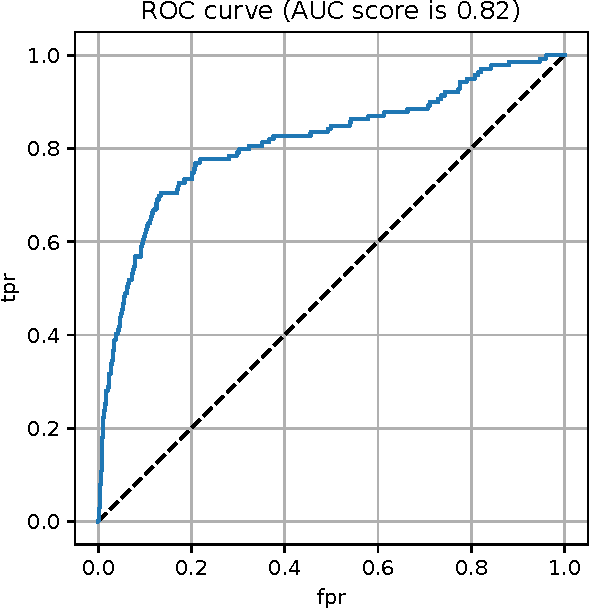
\includegraphics[width=0.35\textwidth]{img/curves_roc}
	\caption{ROC curve. $T\kern-.4exP/P\,\corresponds $ true positive rate (TPR) and $F\kern-.4exP/N\,\corresponds$ false positive rate (FPR)}
\end{figure}

\only<1>{
The higher the area under the curve (ROC AUC) the better the classifier.

\question{What does the dashed diagonal line represent?}

}
\only<2>{

\textbf{But} at the end of the day I need to pick an operating point \notesonly{(i.e. one threshold value)}.

\question{What criterion could I use to favor one threshold over another?}
}

\end{frame}

\mode<article>{
- Assign a ``decision cost $\$_{ij}$'' for different classes 
where $\$_{ij}$ denotes the cost of predicting class $C_{i}$ when the true label is $C_{j}$
(cf. lecture slides 1.4)
}

\begin{frame}

What if the proportions in my training set are different from those of the validation/test set? Which metrics are robust to changes in proportions between different splits of the data.\footnote{cf. jupyter notebook on ISIS for a comparison of different metrics under different conditions.}

\pause 

\slidesonly{\vspace{-2mm}}

\begin{figure}[h]
	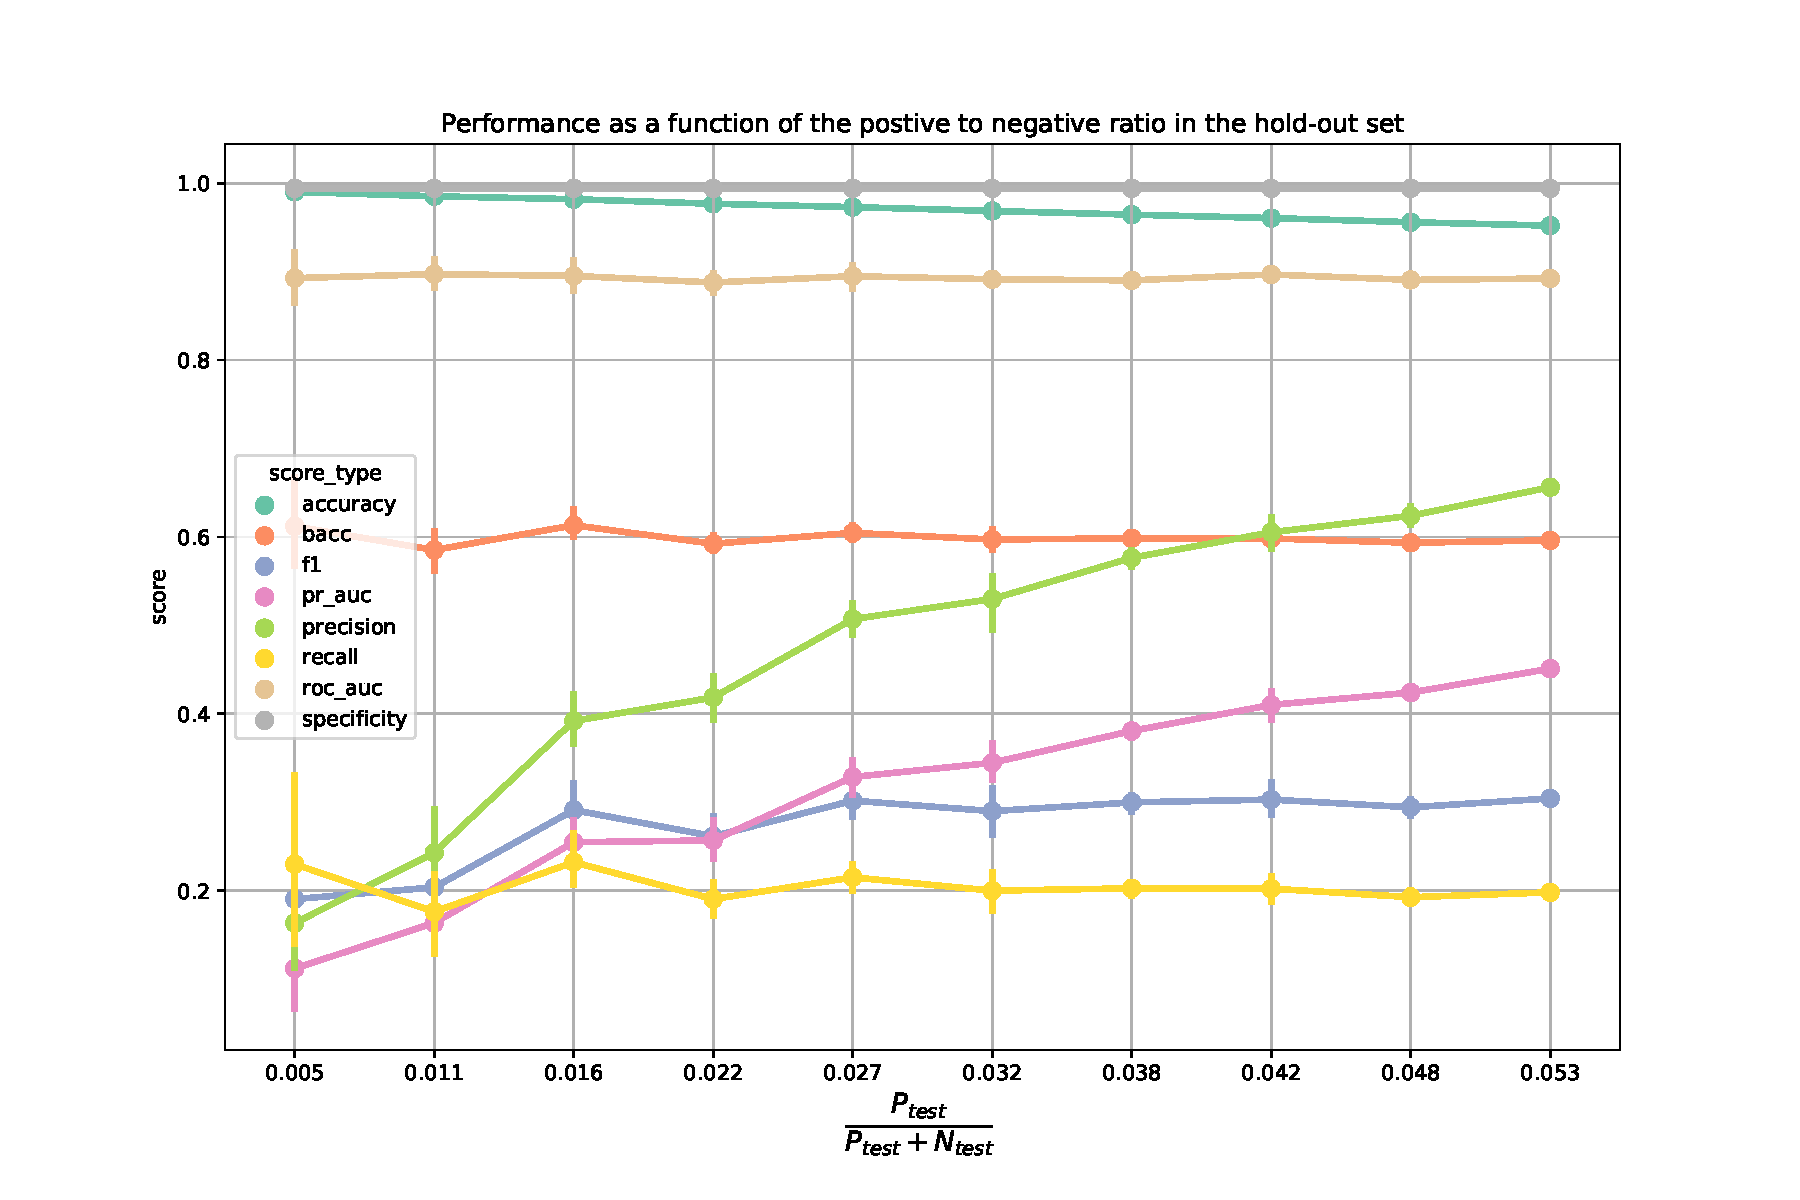
\includegraphics[width=0.8\textwidth]{img/compare_metrics}
	\mode<article>{
	\caption{Comparing metrics under different conditions}
	}
\end{figure}



\end{frame}

\begin{frame}

All we did so far is measure generalization performance and tune our operating point.

\question{Is there anything else we can do about imbalanced data?}

\pause

\begin{enumerate}
\item Train the classifier on a synthetically balanced dataset by
\begin{itemize}
\item sub-sampling from the majority class (no one likes to throw away data)
\item oversampling the minority class
\end{itemize}

\question{Any downsides to oversampling?}

\pause

- the resulting dataset could be too large.
\item class weighted loss function:
e.g. weighted cross entropy:
\begin{equation}
e^{(\alpha)} = -\, \gamma \, y_T^{(\alpha)} \cdot \ln \lbrack y^{(\alpha)} \rbrack - \beta \, (1-y_T^{(\alpha)}) \cdot \ln \lbrack 1-y^{(\alpha)} \rbrack
\end{equation}
where $\beta$ and $\gamma$ represent ``class weights''
\end{enumerate}


\end{frame}
